\documentclass{article}

% packages and configurations
\usepackage{hyperref} % reference chapters
\usepackage{animate} % needed for animations and videos
\usepackage{bm} % bold font in equation environments
\usepackage[utf8]{inputenc}	% für Umlaute ect.
\usepackage{fancyhdr} % für header
\usepackage{lastpage} % für footer
\usepackage{extramarks} % für header und footer
\usepackage{amsthm} % math stuff
\usepackage{amsmath} % math stuff
\usepackage{amssymb} % math stuff
\usepackage{color}
\usepackage[procnames]{listings} % code listings
\usepackage{graphicx} % für graphics
\usepackage[toc]{glossaries} % Glossar
\usepackage{color}
\usepackage{tikz}
\usepackage[absolute,overlay]{textpos} %to translate graphics through space
\usepackage{soul}
\usepackage{xcolor}
\usepackage{textpos}
\usepackage{caption}
\usepackage{parcolumns}
\usepackage{enumerate}
\usepackage[ngerman]{babel} % Umlaute
\usepackage[T1]{fontenc}    % this is needed for correct output of umlauts in pd
\usepackage[section]{placeins} %forces placeins to stay in section
\usepackage{datetime} % custom dates
\usepackage{afterpage}
\usepackage[section]{placeins}

\definecolor{keywords}{RGB}{255,0,90}
\definecolor{comments}{RGB}{0,0,113}
\definecolor{red}{RGB}{160,0,0}
\definecolor{green}{RGB}{0,150,0}

\lstset{language=Python, 
	basicstyle=\ttfamily\small, 
	keywordstyle=\color{keywords},
	commentstyle=\color{comments},
	stringstyle=\color{red},
	showstringspaces=false,
	identifierstyle=\color{green},
	procnamekeys={def,class}}

\title{Bringing together visual analytics and probabilistic programming languages}
\author{Jonas Aaron Gütter  \\
	Friedrich Schiller Universität Jena  \\
    Matrikelnr 152127 \\
    Prof.Dr. Joachim Giesen \\
    M. Sc. Phillip Lucas
	}

\makeglossaries


\begin{document}


\maketitle

\begin{abstract}
A probabilistic programming language (PPL) provides methods to represent a probabilistic model by using the full power of a general purpose programming language. Thereby it is possible to specify complex models with a comparatively low amount of code. With Uber, Microsoft and DARPA focusing research efforts towards this area, PPLs are likely to play an important role in science and industry in the near future.
However in most cases, models built by PPLs lack appropriate ways to be properly visualized, although visualization is an important first step in detecting errors and assessing the overall fitness of a model. This could be resolved by the software Lumen, developed by Philipp Lucas, which provides several visualization methods for statistical models. PPLs are not yet supported by Lumen, and the goal of the master thesis at hand is to change that by implementing an interface between Lumen and a chosen PPL, so that exploring PPL models by visual analytics becomes possible.
The thesis will be divided into two main parts, the first part being an overview about how PPLs work and what existing PPLs there are available. Out of these, the most appropriate one will be chosen for the task. The second, more practical part will then document the actual implementation of the interface.

\end{abstract}

\tableofcontents

\newglossaryentry{Bayesian network}
{
  name=Bayesian network,
  description={...}
}

\newglossaryentry{conditional probability distribution}
{
  name=conditional probability distribution,
  description={...}
}

\newglossaryentry{inference algorithm}
{
  name=inference algorithm,
  description={is a key part of a \gls{probabilistic reasoning system}}
}

\newglossaryentry{joint probability distribution}
{
  name=joint probability distribution,
  description={...}
}

\newglossaryentry{marginal distribution}
{
  name=marginal distribution,
  description={...}
}

\newglossaryentry{probabilistic model}
{
  name=probabilistic model,
  description={is a key part of a \gls{probabilistic reasoning system}}
}

\newglossaryentry{probabilistic programming}
{
  name=probabilistic programming,
  description={is something}
}

\newglossaryentry{probabilistic programming language}
{
  name=probabilistic programming language,
  description={is used to create a \gls{probabilistic reasoning system} more effectively than with a conventional programming language}
}

\newglossaryentry{probabilistic reasoning system}
{
  name=probabilistic reasoning system,
  description={consists of a \gls{probabilistic model} and an \gls{inference algorithm}}
}

\newglossaryentry{Turing-complete}
{
  name=Turing-complete,
  description={a turing-complete machine can perform any computation that could theoretically performed by any computer. universally programmable.}
}
\printglossaries
\section{Road Map}

\begin{enumerate}
	\item Getting started
	\begin{itemize}
		\item set up Master thesis document
		\item Probabilistic Programming Languages
		\begin{itemize}
			\item play at least with: PyMC3, Stan
			\item read the docs, wiki, ...
			\item download the libraries
			\item reproduce the getting started tutorials
			\item --> understand the ideas and how to use it, get a feeling for it
		\end{itemize}
		\item theoretic background: Read Bayesian Data Analysis part I, Chapter 1,2 and part II, chapter 6,7
		\item Lumen
		\begin{itemize}
			\item install locally and play with
			\item understand main idea of Lumen and what we want to do with it
		\end{itemize}
		\item Start filling up your MA thesis document
		\begin{itemize}
			\item understand and write down in MA thesis the "why \& what"
			\item describe the background of the work, e.g. summarize PPLs
		\end{itemize}
		\item give a short presentation
		\begin{itemize}
			\item what have you done and learned
			\item what do you plan to do?
			\item why is it relevant?
			\item how do you plan to measure the success?
		\end{itemize}	
	\end{itemize}
	\item First connection of PPLs to Lumen
	\begin{itemize}
		\item Start from small, very simple and specific example. Generalize later.
		\item Choose PPL to work with
		\begin {itemize}
		\item work out requirements on PPL
		\item work out preferred features of PPL
		\item choose a PPL based on these requrements and preferences
	\end{itemize}
	\item design wrapper of PPL with Lumen
	\begin{itemize}
		\item work out requirement and interface
		\item identify necessary work on Lumen
		\item identify necessary work
	\end{itemize}
	\item Connect chosen specific example with lumen
	\item Continue to work on your master thesis document!
\end{itemize}
\item Improve, generalize and clean up the connection of your PPL to Lumen
\end{enumerate}

\section{Introduction}

\textit{In this section, the motivation for the thesis is explained, the task of the thesis is made clear. Furthermore, the structure of the thesis is outlined here. It is possible to get the basic ideas and results of the thesis from reading only this section and the conclusion.}

\section{Concepts of Bayesian Statistics}

\textit{Theoretical concepts of building statistical models using a Bayesian approach are explained in this section. Also graphical model checking is treated here, as that will be the common use case for the Lumen interface created in this thesis.}
\\
\\
%In the field of statistics, one deals usually with the following questions:
%
%\begin{itemize}
%	\item What kind of model should I choose?
%	\item Which features should I include in my model?
%	\item What are the most likely values for my model parameters?
%	\item What is the most likely outcome for additional observations under certain conditions?
%	\item How certain am I that my estimated parameter values are correct?
%\end{itemize}
%The latter three of these questions can be answered by using a Bayesian approach to statistics. Given a model, Bayesian statistics is about computing a joint probability distribution over all parameters and outcomes, so that a probability density for each possible value of parameters and outcomes can be obtained. Prior knowledge of the problem as well as observed data affect the form of the joint probability distribution. Using marginalization, conditional probability distributions can then be calculated for the desired outcomes. These conditional probability distributions are also called posteriors and can be used for parameter estimation, prediction and assessing the uncertainty of estimates. This chapter will outline how Bayesian statistics are applied to answer the abovementioned questions.
\subsection{Rules of Probabilistic Inference}

When working with Bayesian models, it will be necessary to transform conditional, marginal and joint distributions into one another. There are three rules of probabilistic inference which achieve this: The chain rule, the total probability rule, and the Bayes' rule. The following explanations are taken from \cite{9781617292330}.

\subsubsection{Chain rule}

The chain rule is used to calculate a \gls{joint probability distribution} of several variables from local \gls{conditional probability distribution}s of these variables:

\begin{equation}
P(X_1 ,X_2 ,...X_n ) = P(X_1 )P(X_2 | X_1 )P(X_3 | X_1 ,X_2 )...P(X_n | X_1 ,X_2 ,...X_{n-1}) )
\end{equation}

\subsubsection{Total probability rule}

The total probability rule calculates the probability distribution over a subset of variables, also called a \gls{marginal distribution}, by summing out all the other variables, that is by summing the probability distributions for each combination of values of these variables:

\begin{equation}
P(\boldsymbol X |\boldsymbol Z ) = \sum_{\boldsymbol y}   P(\boldsymbol X ,\boldsymbol Y =\boldsymbol y |\boldsymbol Z )
\end{equation} 

\subsubsection{Bayes' rule}

Bayes' rule calculates the probability of a cause, given an effect, by using the prior probability of the cause and the probability of the effect, given the cause. 

\begin{equation}
P(X|Y) = ( P(Y|X) * P(X) ) / P(Y)
\end{equation}

\subsection{General principle}
Goal of Bayesian Statistics: Setting up a probability model over model parameters and observed data

When doing Bayesian data analysis, we have observed data $Y$ and a prior belief $P(\theta)$ about the mechanism that generated the data, and we use those to set up a full probability model $P(y,\theta|Y)$ over all model parameters $\theta$ and all possible data $y$. The conceptual difference to conventional Statistics is two-fold: First, we don't use prior beliefs in conventional Statistics (at least not for parameter estimation), second, in conventional Statistics we only set up a probability model over the data, not over the model parameters. The model parameters in conventional Statistics are fixed after the parameter estimation.
\\
\\
The principle of setting up the full probability model of Bayesian Statistics (also called the joint probability distribution) is as follows:
\\
According to the chain rule, we can compute the full probability model with the following formula:
\begin{equation}
p(y,\theta|Y) = p(y|\theta,Y) * p(\theta|Y)
\end{equation}
Since the probability for a specific value of $y$ does not depend on the observed data $Y$, if we already know $\theta$, we can write equivalently:
\begin{equation}
p(y,\theta|Y) = p(y|\theta) * p(\theta|Y)
\end{equation}
$p(y|\theta)$ is usually easy to compute since it is given by the chosen model class. For computing the second term, $P(\theta|Y)$, we use the Bayes rule:
\begin{equation}
p(\theta|Y) = p(Y|\theta) * p(\theta) / p(Y)
\end{equation}
This is where the prior belief comes into play.  $p(\theta)$ represents the prior belief, the distribution over the model parameters $\theta$, that we assume from prior knowledge. $p(Y|\theta)$ is the likelihood: The probability that the observed data occur at a given parameter. The problems of choosing a suitable likelihood and prior are treated in sections \ref{Choosing an appropriate prior distribution} and \ref{Sampling distribution}. $p(Y)$, the overall probability of the observed data, does not have to be computed since it can be treated as a constant. (TODO: UNDERSTAND THIS BETTER, HOW p(Y) CAN BE IGNORED)

\subsection{Choosing an appropriate prior distribution}
\label{Choosing an appropriate prior distribution}
There are two interpretations of prior distributions. The \textit{population} interpretation, where the prior distribution is thought of as a population of possible parameters, from where the current parameter is drawn. This, as far as I understand, requires the range of possible values to be known, e.g from past experience. On the other hand, the \textit{state of knowledge} interpretation looks at the prior distribution as an expression of the user's knowledge or uncertainty, so that the assumption is plausible, that the real parameter value is taken from a random realization of the prior distribution.
\\
When we have lots of knowledge about the parameter already, it makes sense to choose an \textit informative prior, which has a big influence on the posterior distribution.On the other hand, if one does not want prior beliefs to affect the outcome of an analysis, one should not choose informative priors, even when lots of knowledge is available. E.g. when testing a hypothesis, it is not wise to include information in the prior that supports the hypothesis for fairness reasons(?? look that up again on p. 56.). If there is no sufficient data to estimate a prior, it is desirable to choose a prior that is \textit noninformative, meaning that it will contribute very little to the posterior distribution ('let the data speak for itself'). A common noninformative prior, motivated by Laplace's principle of insufficient reason, is the uniform distribution. However, the uniform distribution is not ideal since it is dependent on the parametrization: Applying a uniform distribution to $p(x)$ leads to a non-uniform distribution when looking at $p(x^2)$ and the other way round \cite{1439840954}. Jeffrey's approach to find noninformative prior distributions negates this problem by choosing a prior that is invariant to the parameterization (see https://eventuallyalmosteverywhere.wordpress.com/2013/05/10/bayesian-inference-and-the-jeffreys-prior/).
Besides informative and noninformative prior distributions there is also the \textit {weakly informative} prior distribution. This kind of prior does affect the posterior distribution in terms of regularization (e.g. it prevents extreme outliers), but it does not contain any further special knowledge about the parameter. A normal distribution with high variance is often used as weakly informative prior.
\\
The parameters of the prior distributions are called hyperparameters. The property that prior and posterior distribution are of the parametric form (e.g., both are a beta distribution) (for a given likelihood distribution), is called conjugacy. Conjugate prior distributions have the advantages of being computationally convenient and being intertpretable as additional data.
\\
A prior distribution is called \textit{proper} if it does not depend on data and sums to 1 \cite{1439840954}. Proper distributions can be normalized. The uniform prior for example is \textit{improper}, since it can't be normalized.

\subsection{Sampling distribution}
\label{Sampling distribution}

The sampling distribution, also called the likelihood of the data.
\\
Often it is about which distribution class should be chosen for the prior and the likelihood. Standard, convenient distributions for single-parameter models: normal, binomial, Poisson, exponential. Those can also be combined to represent more complex distributions. For different classes of sampling distributions there are corresponding conjugate prior distributions which lead in turn to posterior distributions of the same form. \cite{1439840954}
\\
distributions can be chosen for mathematical convenience. One could estimate hyperparameters of the likelihood distribution from the data in some cases. This is a bit of a circular reasoning, but apparently  it is appropriate for \cite{1439840954}.

\subsection{Evaluating models}

Since ``all models are wrong", it is necessary, after a Bayesian model has been found, to capture the extent to which the model fails to describe reality. In Bayesian analysis, both the prior and the likelihood distribution can be sources of error.

Different models can lead to different posterior inferences, even if both models have a good fit.

model checking: How good does the model fit the data?
Sensitivitiy analysis: Comparison of different models with good fit

This is necessary after a joint probability density and a posterior density are calculated. How good are the prior and the likelihood model?
\textit{Sensitivity analysis} deals with the question, how much the posterior is changed when one chooses a different (but also reasonable) model for the likelihood or the prior, or other assumptions affecting the posterior.

In theory: Setting up a 'super-model' as joint-distribution which includes all possible realities. Posterior of this super-model then automatically incorporates the sensitivity analysis. In practice this is conceptually and computationally infeasible and also is still dependent on the assumptions made when creating the super-model being correct.

One way is just to compare model predictions with the actual outcomes (this is referred to as external validation). If for some reason it is not possible to get the acutal outcomes (for example if they lie in the future), one needs to approximate external validation with the available data.

\textit{Posterior predictive checking}: Use global summaries of the data distribution and the predictive distribution to evaluate the model: Draw random samples from the predictive distribution, compare e.g. the smallest of these values with the smallest value in the data...

model checking by calculating \textit{test quantities}. \textit{test quantities} are scalar summaries of parameters that are used to compare data to simulations. \textit{test quantities} are similar to test statistics in the classical approach. Besides on the data, \textit{test quantities} can also depend on the parameters.

Graphical comparison of simulated and data histograms (!! maybe here point out usefulness of Lumen)

tail-area-probability: p-value. p-value in classical statistics: Probability, that, given a parameter $\theta$, a test statistic for replicated data is greater or equal the test statistic for the observed data,as shown in equation \ref{eq:classical_p}:

\begin{equation}
p_C = Pr(T(y^{rep}) >= T(y) | \theta)
\label{eq:classical_p}
\end{equation}

\cite{1439840954}

The Bayesian p-value, on the other hand, is not conditional on a fixed $\theta$, since in Bayesian statistics parameters are drawn from a distribution the same way as outcome variables. Instead, the observed data $y$ is the fixed quantity for the Bayesian p-value, as shown in equation \ref{eq:bayesian_p}

\begin{equation}
p_B = Pr(T(y^{rep},\theta) >= T(y,\theta) | y)
\label{eq:bayesian_p}
\end{equation}

p-value depends on the chosen test quantity.


Bayesian predictive checking: choose and compute test quantites for the data and for simulations, then compute the p-value for the test quantity (probability that the test quantity of the data could have arisen under the model)

Test quantities give information about a specific aspect of the observed/simulated data. A model can predict values that are in some aspects similar to the data, in other aspects different. Therefore it can make sense to compute p-values fur several different test quantities.
If a test quantity is dependent on the model parameters it has to be simulated both for the observed as well as for the predicted data. This makes it possible to compare both test statistics (for observed and for simulated values) pointwise, eg. in a scatterplot or in a histogram of the differences. The scatterplot should be symmetric around the 45 degree line, the histogram should include 0 (and be symmetric around 0??).
Test quantities are most useful when they measure an aspect that is not directly recognizable in the probability model.
Graphical visualization can be used to identify useful test quantities.
If a test quantity has a p-value close to 0 or 1, the aspect that is analysed by the test quantity is not well captured in the model.
\\
Model checking depends on the data-collection model (how the data was collected), since data has to be replicated for computing a p-value. Posterior Inference however does not depend on the data collection model, as long as the likelihood model stays the same. Because of this, the same posterior results(what are the parameters) can get different model checking results (how well does the model fit) when the data-collection model is changed.
\\
Marginal predictive checks: Instead of replicating data from the joint posterior distribution, one can also compute the probability for a certain outcome, and compare this probability with the data....(p.153).
\\
Graphical posterior predictive checks: Basic Idea: Visualize the data alongside simulated data and so find discrepancies --> perfect in Lumen 
Possibilities:
\begin{itemize}
	\item Direct display of all the data
	\item Display of data summaries (e.g. if the data is so large that it is not helpful to display all the data)
	\item Display a measure of discrepancy betweem model and data
\end{itemize}

MAYBE BUILD EXAMPLES WITH LUMEN TO ILLUSTRATE USEFULNESS OF LUMEN
\paragraph{Direct data display}

Show the complete data and its correspondent simulations. It's best to show several replications.

\paragraph{Display data summaries}

\paragraph{Display discrepancy measures}
Bayesian residuals are defined by $y_i - g(x,\theta)$, where, in contrast to classical residuals, $\theta$ is not a point estimate of parameters, but a single draw from the posterior distribution of the parameters.

Difficult with discrete data, since residuals can only take certain discrete values. Graphical visualization can then be misleading since the discrete values can suggest patterns. To avoid this, one can use \textit{binned residuals}, that is plotting the averages over a number of residuals and their corresponding outcomes. 



%\subsection{Stuff that has to be/could be placed somewhere}
%
%
%\subsubsection{Posterior distribution}
%
%The posterior distribution is a compromise between the prior distribution and the sample distribution, with the prior distribution becoming less important as the sample size increases \cite{1439840954}.
%posterior distributions can be described numerically by mean, median, modes. The uncertainty can be described by quantiles. The highest posterior density region is also a possibility, it is the area that for example contains 95\% of the posterior probability density, like quantiles, but has the additional constraint that the density on each point inside the area has to be bigger than the density on any point outside the area. It does not have to be one single connected area  \cite{1439840954}.
%\\
%For the posterior distribution, a normal distribution is often assumed.
%
%\subsubsection{Drawing inference}
%According to \cite{Wang2018}, the likelihood of a new datapoint can be calculated by integrating the product of the prior likelihood and conditional probability of $\beta$ over the space of $\beta$, as shown in equation \ref{eq:posterior_predictive}. This formula can also be derived using the chain rule (I think).
%\\
%Making predictions for a new data points requires both the probability distribution of the new data point, given a parameter value, as well as the probability distribution of the parameter, given the old data points.
%\\
%If it is not possible to perform calculations directly from the posterior distribution (e.g. if there is no closed form but only a discrete approximation of the posterior distribution), one can simulate data points from the posterior distribution instead and perform calculations on them \cite{1439840954}.
%
%\begin{equation}
%p(x_{new}|\boldsymbol x, \alpha) = \int p(x_{new}|\beta) * p(\beta | \boldsymbol x,\alpha) d \beta
%\label{eq:posterior_predictive}
%\end{equation}

\subsection{Gibbs Sampling}

Gibbs Sampling assumes that we don't know the joint posterior distribution $p(\theta_0,...,\theta_n)$, but we do know the conditional distribution $p(\theta_i | \theta_j, j \neq i)$ for each quantity.
Algorithm works as follows:
\begin{itemize}
\item Select arbitrary starting points for $\theta_0,...,\theta_n$
\item Update each $\theta$ by drawing from its conditional distribution given the values of the other quantities. Repeat this step until terminate condition is fulfilled.
\end{itemize}
\cite{Martz1994}

\section{Probabilistic Programming}

\textit{In this section,  the idea of Probabilistic Programming is explained. It is defined what a Probabilistic Programming Language is, and a number of PPLs are introduced. A focus is laid on the abilities of the PPLs for graphical model checking}
\\
\\
"Probabilistic programming is an emerging paradigm in statistical learning, of which Bayesian modeling is an important sub-discipline." \cite{Salvatier2016}
\\
stochastic data types (--> probability distributions) make it easier to perform bayesian data analysis

\subsection{What are Probabilistic Programming Languages}

Modelle spezifizieren/beschreiben 

Random Variables can be represented as objects
\\
Posterior probability for parameters comes from the Bayes formula: $P(\theta|data) = p(data|\theta) * p(\theta) / p(data)$. The marginalized probability of the data $p(data)$ is given as follows:
$p(data) = \int p(\theta,data) d \theta$. This integral can't be calculated (TODO: UNDERSTAND THAT BETTER), so PPLs instead sample from this distribution and get their inference from the samples.



\cite{wiki:Probabilisticprogramminglanguage}

effizienter in der Beschreibung von Modellen als herkömmliche Programmiersprachen \cite{Hardesty2015}

unifying general purpose programming with probabilistic modeling \cite{probabilistic-programming.org}


A \gls{probabilistic reasoning system} uses prior knowledge in the form of a \gls{probabilistic model} to answer a certain query. The particular propertes of the query as well as the prior knowledge are given to an \gls{inference algorithm} which returns an answer in the form of probabilities. Example is shown in figure \ref{fig:example_prs}. Probabilistic Programming is the implementation of a \gls{probabilistic reasoning system} by using a programming language.

Traditional means for representing models are not always sufficient for probabilistic models. Therefore, probabilistic programming languages were introduced to be able to represent models with the full power of a programming language (http://www.probabilistic-programming.org/wiki/Home).


\begin{figure}
	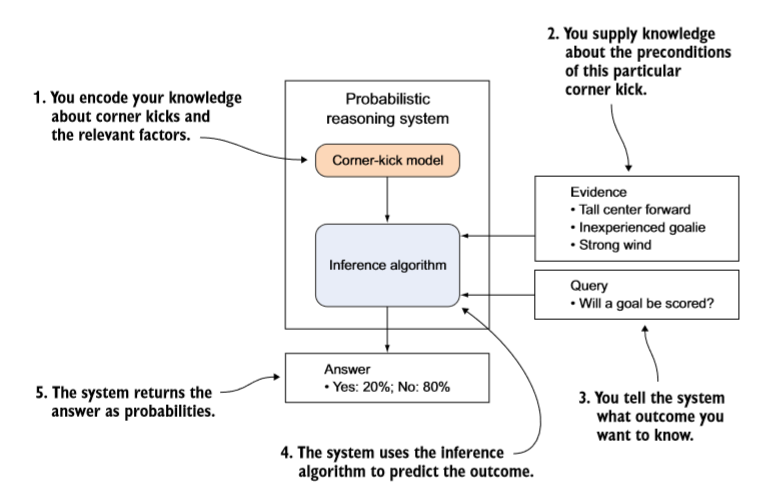
\includegraphics[width=\textwidth]{images/probabilistic_reasoning_system.PNG}
	\caption[General workflow example of a probabilistic reasoning system. Source: \cite{9781617292330}]{General workflow example of a probabilistic reasoning system}
	\label{fig:example_prs}
\end{figure}

\subsection{Inference through sampling}

Using the Bayes formula, we get the posterior distribution the following way:

\begin{equation}
	p(\theta|x) = p(x|\theta) * p(\theta) / p(x)
\end{equation}
We get both the likelihood $p(x|\theta)$ and the prior $p(\theta)$ from the model assumptions. The marginalized probability over the data, however, is more complicated. To compute it analytically, we would have to compute the following integral:

\begin{equation}
\begin{split}
	p(x) = \int p(\theta,x) d \theta \\
		 =  \int p(x|\theta) * p(\theta) d \theta
\end{split}
\end{equation}
Calculating this integral can be very difficult or impossible, since the integral can be multidimensional. So, it is not possible to get the posterior distribution of the parameters analytically. However, there are methods to sample exactly from the posterior distribution of the parameters. The easiest of them is called Simple Monte Carlo. There
we approximate the integral by sampling over the likelihood and the prior and then taking the mean over the samples:
\begin{equation}
	\int p(x|\theta) * p(\theta) d \theta \approx 1/m * \sum^m p(x|\theta_i),\quad \theta_i \sim p(\theta)
\end{equation}
Simple Monte Carlo has a number of disadvantages, so more sophistically methods are genrally used, like Gibbs sampling or NUTS.

Markov Chain simulation: 

Parameter values are drawn sequentially from an approximate distribution. In each sequence, the values depend only on the values of the preceding sequence (and maybe on the index of the sequence), which makes those draws a markov chain.

So in each step, values are drawn from a transition distribution $T_t(\theta^t|\theta^{t-1})$.

The chain has the property of becoming more similar to the real posterior distribution of the parameters in each iteration.

\subsection{Difference to conventional Programming Languages}

When estimating parameters, not only the most likely value for the parameters is given, but also their uncertainty.

\subsection{Comparing Different Probabilistic Programming Languages}

\begin{itemize}
	\item stan for python: https://pystan.readthedocs.io/en/latest/
	\item pymc3: https://docs.pymc.io/notebooks/getting\_started.html\#Case-study-2:-Coal-mining-disasters
	\item edward: http://edwardlib.org/getting-started
	\item pyro: http://pyro.ai/
\end{itemize}

\subsubsection{Stan for python}

Stan is an open-source program written in C++ that is designed for Bayesian inference on user-specified models. It consists of the following components:
\begin{itemize}
	\item A modeling language that allows users to specify custom models
	\item An inference engine which uses Hamilton Monte Carlo methods for sampling to get an approximation for the posterior distribution
	\item An L-BFGS optimizer for finding local optima
	\item Procedures for automatic differentiation which are able to compute gradients required by the sampler and the optimizer
	\item Routines to monitor the convergence of parallel chains and compute inferences and effective sample sizes
	\item Wrappers for Python, R, Julia and other languages
\end{itemize}
The code for describing a model by using the aforementioned modeling language is divided into six blocks: \textit{data}, \textit{transformed data}, \textit{parameters}, \textit{transformed parameters}, \textit{model}, and \textit{generated quantities}: In \textit{data} and \textit{transformed data}, the structure of the input data, along with any constraints, is given. The difference between the former and the latter is that variables in \textit{transformed data} are functions of other data variables, whereas variables in \textit{data} are not. For example if in \textit{data}, a variable $x$ is listed, then in \textit{transformed data} one can specify a variable $y=x^2$. In \textit{parameters} and \textit{transformed parameters}, the parameters of the models are described, whereat, as in the data blocks, the latter contains variables that are functions of other parameters. In \textit{model}, the model structure in the form of prior and likelihood distributions is given. Finally, the block \textit{generated quantities} can be used to perform simulations and make predictions. In \ref{fig:stan_example_code}, an example from \cite{Gelman_2015} is shown, where the model $y=a_1e^{-b_1x} + a_2e^{-b_2x}$ is fit to data, using the PyStan interface of Stan for Python. Since not all of the aforementioned blocks are mandatory, only four of them are used in the example.
\\
PyStan also provides basic plotting methods for the posterior distributions of the parameters.

is not able to perform inference on discrete parameters. Discrete data and discrete-data models, however, are possible

computes the log-posterior density

\cite{Gelman_2015}

\cite{Hoover2016}

für den Code evtl. https://github.com/stephen-hoover/presentations zitieren

\begin{figure}
	\begin{lstlisting}
	# Specify model
	example_code = """
	data {
	// Define input data in this block
	int N;
	vector[N] x;
	vector[N] y;
	}
	parameters {
	// These are random parameters which we want to estimate
	vector[2] log_a;
	ordered[2] log_b;
	real<lower=0> sigma;
	}
	transformed parameters {
	// Create quantities derived from the parameters.
	vector<lower=0>[2] a;
	vector<lower=0>[2] b;
	a <- exp(log_a);
	b <- exp(log_b);
	}
	model {
	// Define your model here
	vector[N] ypred;
	ypred <- a[1]*exp(-b[1]*x) + a[2]*exp(-b[2]*x);
	y ~ lognormal(log(ypred), sigma);
	log_a ~ normal(0,1); 
	log_b ~ normal(0,1);
	}
	"""
	
	# Pass data to the model. x and y are the observed data
	example_dat = {'x':x,'y':y,'N':len(x)}
	# Fit model
	sm = pystan.StanModel(model_code=example_code)
	fit = sm.sampling(data=example_dat, iter=1000, chains=4)
	print(fit)
	\end{lstlisting}
	\label{fig:stan_example_code}
	\caption[Example code of a simple Bayesian model using Stan]{Example code of a simple Bayesian model using Stan}
\end{figure}

\subsubsection{Pymc3}

PyMC3 is an open-source probabilistic programming framework for Python. The following explanations are taken from \cite{Salvatier2016}. Specification of Bayesian models in PyMC3 is done by encoding the prior, the sampling and the posterior distributions through three types of random variables: Stochastic, deterministic and observed stochastic ones. Stochastic random variables have values which are in part determined randomly, according to a chosen distribution. Commonly used probability distributions like Normal, Binomial etc. are available for this. Deterministic random variables, on the other hand, are not drawn from a distribution, but are calculated by fixed rules from other variables, for example by taking the sum of two variables. Lastly, there are the observed stochastic random variables which are similar to stochastic random variables, except that they get passed observed data as an argument, that should not be changed by any fitting algorithm.  This kind of random variable can be used to represent sampling distributions.
\\
PyMC3 mainly uses simulation techniques to draw inference on posterior distributions. It focuses especially on the No-U-Turn Sampler, a Markov Chain Monte Carlo algorithm, that relies on automated differentiation to get gradient information about continuous posterior distributions. PyMC3 also provides basic methods for plotting posterior distributions.
\\
The code piece  in \ref{fig:pymc3_example_code} shows a simple example of a Bayesian model, taken from \cite{Salvatier2016}. There, the data X1, X2 and Y is used to fit a regression model. First, prior distributions for the model parameters are set up as stochastic random variables, then the regression model itself is specified by a deterministic random variable and lastly the sampling distribution is described by an observed stochastic random variable to which the observed outcome Y is given as a parameter. Finally, the posterior distribution is simulated by drawing 500 samples from it.

\begin{figure}
	\begin{lstlisting}
	import pymc3 as pm
	
	basic_model = pm.Model()
	
	with basic_model:
	# describe prior distributions of model parameters. Stochastic variables
	alpha = pm.Normal('alpha', mu=0, sd=10)
	beta = pm.Normal('beta', mu=0, sd=10, shape=2)
	sigma = pm.HalfNormal('sigma', sd=1)
	# specify model for the output parameter. Deterministic variable
	mu = alpha + beta[0]*X1 + beta[1]*X2
	# likelihood of the observations. Observed stochastic variable
	Y_obs = pm.Normal('Y_obs', mu=mu, sd=sigma, observed=Y)
	
	# model fitting by using sampling strategies   
	with basic_model:
	# draw 500 posterior samples
	trace = pm.sample(500)
	pm.summary(trace)
	\end{lstlisting}
	\label{fig:pymc3_example_code}
	\caption[Example code of a simple Bayesian model using PyMC3]{Example code of a simple Bayesian model using PyMC3}
\end{figure}

strictly positive priors are transformed with log transformation, so that they are unconstrained, since that is better for sampling

There is the possibility to create own theano functions in python. Gradient based sampling methods don't work for user-defined functions however, except when a gradient is explicitly added.

Similarily pmc3 allows to define own distributions
\subsubsection{Edward}

\subsubsection{Pyro}
\subsubsection{BUGS and Jags}
mentioned in \cite{Gelman_2015}
based on graphical models

\section{Lumen}

\textit{In this section, the Software Lumen is introduced and its abilities and uses are elucidated, especially its potential uses for Bayesian model checking in conjunction with PPLs. This covers also the theoretical aspect: Which distribution do we want to visualize with Lumen and how do we get it (using the formula $P(y,\theta|Y) = P(y|\theta) * P(\theta|Y)$)? It is outlined, what the goal of the thesis is precisely, in other words what possibilities should the interface ideally give to a user who has written a model with a PPL. Too achieve this is goal it is necessary to understand how Lumen works, so the functionality of Lumen is also explained here.} 
\\
The overall goal of the thesis is to build an API, that makes it possible to a PyMC3 (or other PPL) user to get his model visualized in lumen with minimal effort. For example it would be good if one just has to call one function with a PyMC3 model as parameter to transport the model into the lumen frontend.
\\
uses modelbase as backend: modelbase is a python package that provides means for fitting models to data and manipulate models by marginalization and conditionalization.
\\
model classes are in \url{modelbase/mb_modelbase/models_core}
data is in \url{mb_data}. model fitting is done in the script fit\_models.py, which is also in \url{mb_data}. The corresponding model class has to be imported, the models have to be 'registered' in the known\_models variable and then the models to be fit have to be listed in the variable debugincl.

 Fitted models that can be accessed by lumen are then stored in \url{data_models}.

\subsection{Functionality}

In the modelbase repository, a model class is described by a python file that includes a class with several prescribed methods \url{https://ci.inf-i2.uni-jena.de/gemod/modelbase/blob/master/mb_modelbase/models_core/models.py} is a template for such a model class file, where all important methods are explained.
\\
In the mb\_data repository, data that can be used for model fitting is contained. It has a file named fit\_models.py that contains specifications of data and corresponding models. It can be called with one of these specifications to create a mdl file. In the directory data\_models all mmdl files are currently stored that can be displayed by the lumen frontend.
\\
The first step would be to implement a model there that is built by using a PPL. Then make sure that all necessary methods are correctly implemented and the visualization works as expected. One of the advantages of PPLs is the flexibility of the models specified, which is nullified by describing one fixed model. Therefore, the next steop is about thinking about a possibility to pass more flexible models. Maybe a function where you just give a model object as input that then automatically generates the necessary methods for the use in lumen??  Other possibilities? (would be good to ask that at the presentation)




compare to the plotting methods of PyMC3 / Stan

\subsection{Requirements for a PPL}

possible criterium: variety of distributions that can be described?



\section{Konzept/Planung}

In Bayesian data analysis we have a prior distribution for the parameters, $p(\theta)$, which represents our knowledge about them without seeing any data. We have also the likelihood of our data, $p(X|\theta)$, which represents the probability of obtaining the data $X$ given the parameter $\theta$. Using the Bayes' rule, we can then compute the posterior distribution for $\theta$, $p(X|\theta)$:

\begin{equation}
p(\theta|X) = p(X|\theta) * p(\theta) / p(X)
\end{equation}

Since the posterior distribution for $\theta$ can often not be computed analytically, Probabilistic Programming Languages use sampling methods to approximate the posterior distribution for $\theta$.

When we want to visualize parameters and data, and also want to condition and marginalize arbitrarily, we need the joint distribution $p(x,\theta|X)$. The joint distribution can be computed by:

\begin{equation}
p(x,\theta|X) = p(x|\theta) * p(\theta|X)
\end{equation}

The posterior distribution of the parameters, $p(\theta|X)$, can be approximated by PPLs through sampling, as stated above. (--> Make sure that this is true!!). To get density values from samples, we have to perform density estimation methods \url{http://scikit-learn.org/stable/modules/generated/sklearn.neighbors.KernelDensity.html#sklearn.neighbors.KernelDensity.score_samples}

\subsection{Complete example of a simple Bayesian model}
\label{subsec: Complete example of a simple Bayesian model}

To get a sort of ground truth, a Bayesian model is fitted first without the use of a PPL. To check if a PPL is deployed correctly, the same model can be fitted by a PPL. The results of the PPl approach and the ground truth should then look the same.
\\
Assume we want to fit a model with the two dimensions $x$ and $mu$, one of them, $x$, we can observe, the other one, $mu$, we can't observe. Furthermore we assume the following priors:
\begin{equation}
\begin{split}
mu &\sim N(0,1)\\
x &\sim N(mu,1)
\end{split}
\end{equation}
Assume again, that we observe some data $X$ of the observable dimension $x$.
We now want to compute the joint posterior distribution of both dimensions $mu$ and $x$, conditioned on the observed data $X$.
This distribution is computed as follows:
\begin{equation}
\begin{split}
&P(x,mu|X) \\
= &P(x|mu,X) * P(mu|X) \\
= &P(x|mu) * P(mu|X) \\
= &P(x|mu) * P(X|mu) * P(mu) / P(X) \\
= &P(x|mu) * P(X|mu) * P(mu) / \int P(X,mu) \hspace{1mm} d \hspace{1mm} mu \\
= &P(x|mu) * P(X|mu) * P(mu) / \int P(X|mu) * P(mu) \hspace{1mm} d \hspace{1mm} mu
\end{split}
\end{equation}
The data $X$ is generated as follows:\\
\begin{figure}[h]
	\begin{lstlisting}
	import pymc3 as pm
	import numpy as np
	import pandas as pd
	import matplotlib.pyplot as plt
	from pylab import *
	from scipy.stats import norm
	import scipy.integrate as integrate
	
	# Generate data
	np.random.seed(1)
	size = 100
	mu = np.random.normal(0,1,size=size)
	sigma = 1
	X = np.random.normal(mu,sigma,size=size)

	\end{lstlisting}
	\label{fig:groundtruth_example_code_data_generation}
\end{figure}
\\
The necessary distributions leading to the actual joint posterior distribution are written as follows:
\begin{figure}[h]
	\begin{lstlisting}
	def prior_mu(mu):
	density = norm.pdf(mu, loc=0, scale=1)
	return density

	def likelihood_x(x,mu):
	density = norm.pdf(x, loc=mu, scale=1)
	return density

	def likelihood_X(X,mu):
	res = 1
	for point in X:
	res *= likelihood_x(point,mu)
	return res

	def likelihood_times_prior_mu(X,mu):
	return likelihood_X(X,mu) * prior_mu(mu)

	def prior_X(X):
	res = integrate.quad(lambda mu: likelihood_times_prior_mu(X,mu),a=-np.inf,b=np.inf)[0]
	return res

	def joint_posterior(x,mu,X):
	res = likelihood_x(x,mu) * likelihood_X(X,mu) * prior_mu(mu) / prior_X(X)
	return res
	\end{lstlisting}
	\label{fig:groundtruth_example_code_distributions}
\end{figure}
Finally, the joint posterior distribution is visualized, as shown in \ref{fig:ground_truth_posterior_1}.
\begin{figure}
	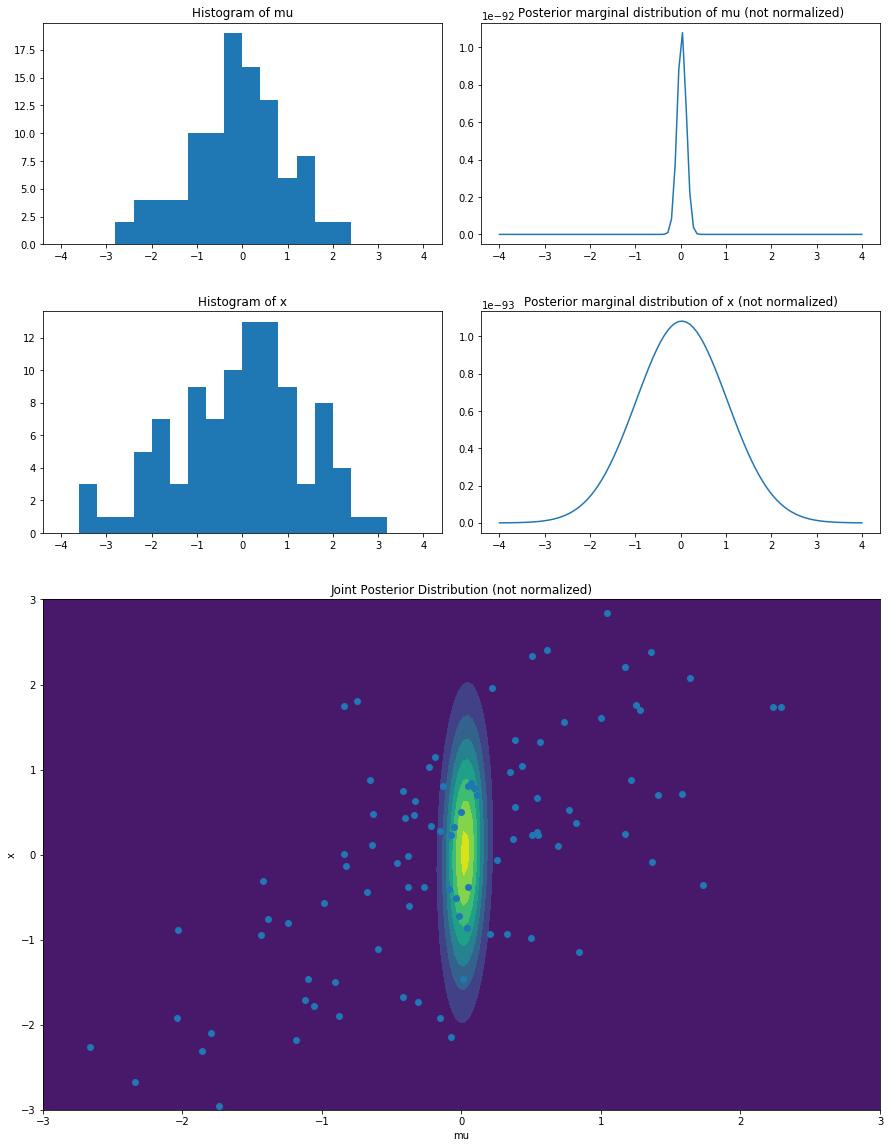
\includegraphics[width=\textwidth]{images/ground_truth_posterior_1.png}
	\label{fig:ground_truth_posterior_1}
	\caption[Posterior distributions of the example model]{Posterior distributions of the example model}
\end{figure}

% Parameters for ground_truth_posterior_1.png:
%# data parameters
%size = 100
%mean_mu = 0
%sigma_mu = 1
%sigma_x = 1
%
%# model parameters
%prior_mean_mu = 0
%prior_sigma_mu = 1
%prior_sigma_x = 1
%
%# plot parameters
%resolution_joint_mu = 200
%resolution_joint_x = 200
%range_joint_mu_upper = 3
%range_joint_mu_lower = -3
%range_joint_x_upper = 3
%range_joint_x_lower = -3
%resolution_marginal_mu = 100
%resolution_marginal_x = 100
%range_marginal_mu_upper = 4
%range_marginal_mu_lower = -4
%range_marginal_x_upper = 4
%range_marginal_x_lower = -4

We see, that $mu$ is very narrowly contained around zero, whereas $x$ has a much broader distribution. A relationship between $mu$ and $x$ is not visible. This is astonishing for me at first: Since I know that $x$ is dependent on $mu$, I would expect this dependency to show up in the visualisation. In other words, I would expect the probability density for a high $mu$ and a high $x$ to be relatively similar to the density of a $mu$ near zero and a high $x$, and to be much higher than the density of a high $mu$ and a low $x$.
Let's look again at the formula:
\begin{equation}
P(x,mu|Y) = P(x|mu) * P(X|mu) * P(mu) / \int P(X|mu) * P(mu) \hspace{1mm} d \hspace{1mm} mu
\end{equation}
To evaluate the abovementioned expectations, it is not necessary to keep the normalizing constant, since a constant does not affect the order of the values. So we keep:
\begin{equation}
P(x,mu|Y) = P(x|mu) * P(X|mu) * P(mu)
\end{equation}
When we consider only the first and the last term of this formula, it behaves exactly as expected: $P(x=high|mu=high)*P(mu=high) = P(x=high|mu=zero)*P(mu=zero)$
and $P(x=high|mu=high)*P(mu=high) >> P(x=low|mu=high)*P(mu=high)$. What was messing with my expectations is the term in the middle, which gives the likelihood of the observed data. For a value of $mu$ that is far from the true mean, that term quickly becomes extremly small, since all the data points speak against it. That's why the distribution is so strongly centered to the middle: All the outer values of $mu$ are getting assigned extremly low density values by this middle term. I still don't quite understand why it is centered \textit{that} strong: The real $mu$ is distributed far wider, with a standard deviation of 1. On the other hand, that could just be a visualization issue.
The dependance between $mu$ and $x$ is in fact still there in the joint posterior distribution, it's just overlapped by the centering effect of the data. If we choose only a very small number of data points, we get the distribution that is shown in \ref{fig:ground_truth_joint_posterior_2}.
\begin{figure}
	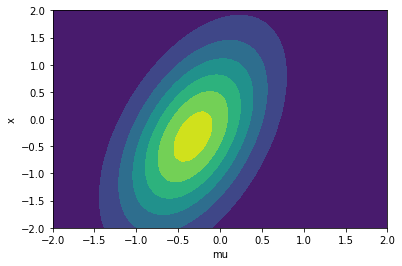
\includegraphics[width=\textwidth]{images/ground_truth_joint_posterior_2.png}
	\label{fig:ground_truth_joint_posterior_2}
	\caption[Joint probability density of the example model with only two data points]{Joint probability density of the example model with only two data points}
\end{figure}
The dependency between the variables is here clearly visible, since the data points do not influence the plot anymore.

To understand this example better, I make changes in the model and or in the data generation and look how those changes affect the posterior distributions. 

Which possibilities are there to change the model? 

number of training points
mean of mu
sigma of mu
sigma of x
prior mean mu
prior sigma mu
prior sigma x

mu is also observed


What do I expect? 

When the variance in both the data generation and the prior for mu increases: the data will be more spread. I expect the $P(X|mu)$-part of the joint posterior to not change, since the data $X$, on the one hand, will be more spread out, which is in favor of smaller density values, but on the other hand, the variance of the prior distribution is also higher, which leads to bigger density values for points far from the mean. The $P(x|mu)$-part will probably contribute to a wider distribution in both dimensions: $P(x|mu)$ for a given $x$ gets assigned a lower probability value in the center and bigger values on the edges, when increasing the variance. The same is true for a given $mu$. The $P(mu)$-part will also contribute to a wider distribution in the $mu$-dimension.
So when increasing the variance, I expect the whole distribution to get wider, especially in the $mu$-direction.

What happens is that the density at each point is exactly zero. Why is this?







Hint: For visualization purposes, it should not be necessary to compute the normalizing constant.

\subsection{PyMC3 example of a simple Bayesian model}
\label{subsec: PyMC3 example of a simple Bayesian model}
The model from chapter \autoref{subsec: Complete example of a simple Bayesian model} is now created by using PyMC3 with the code shown in \ref{fig:PyMC3_example_code_simple_model}.
\begin{figure}[h]
	\begin{lstlisting}
	import numpy as np
	import pandas as pd
	import pymc3 as pm
	import matplotlib.pyplot as plt
	
	# Generate data
	np.random.seed(2)
	size = 100
	mu = np.random.normal(0,1,size=size)
	sigma = 1
	X = np.random.normal(mu,sigma,size=size)

	# Specify model
	basic_model = pm.Model()
	with basic_model:
	sigma = 1
	mu = pm.Normal('mu',mu=0,sd=sigma)
	X = pm.Normal('X',mu=mu,sd=sigma,observed=X)

	# Draw samples from posterior
	nr_of_samples = 100
	with basic_model:
	trace = pm.sample(nr_of_samples,chains=1)
	samples_mu = trace['mu']
	samples_X = np.random.normal(samples_mu,1,size=nr_of_samples)
	\end{lstlisting}
	\label{fig:PyMC3_example_code_simple_model}
	\caption[Code used to specify the example model in PyMC3]{Code used to specify the example model in PyMC3}
\end{figure}
Figure \ref{fig:PyMC3_joint_posterior_samples_simple_model} shows samples from the joint posterior distribution of the fitted model. Similarities in shape to the real joint posterior distribution in \ref{fig:ground_truth_joint_posterior_1} are visible, so it is assumed, that PyMC3 captures the model correctly.
\begin{figure}
	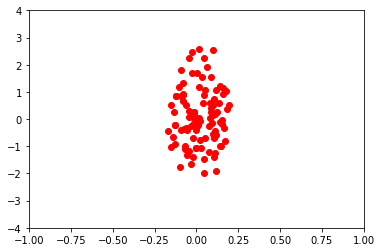
\includegraphics[width=\textwidth]{images/PyMC3_joint_posterior_samples_simple_model.png}
	\label{fig:PyMC3_joint_posterior_samples_simple_model}
	\caption[Samples from the posterior joint distribution of the example model in PyMC3]{Samples from the posterior joint distribution of the example model in PyMC3}
\end{figure}
\section{Practical implementation}

\textit{In this section, the choices and attempts made during the practical implementation of the interface are elucidated. At first, the choice of the PPL is justified.}

My first approach will be to write a fixed probabilistic models as a model class, that fits one specific model to a specific set of data. (linear regression)


simple, fixed example:
In Lumen, several methods have to be specified for a model class to work. The first, which will always be called first, is the method that assigns data to the model.
\\
The second is the method that fits the model to the data. It will always be called second, after the data setting method. In Bayesian statistics, fitting means finding the joint posterior distribution. In the context of PPL, it means drawing samples from all variables, so that the joint posterior distribution can be approximated. The whole model should probably be specified in this method? Or before?
\\
Another method is the one that marginalizes a random variable out. In a Bayesian model, a random variable can be a parameter as well as a data dimension.  What is wanted here is thus the posterior distribution over all variables listed in keep.
In PyMC3, marginalizing means sampling over a subset of the variables. Samples were already drawn in the fitting method, so only the corresponding columns of those samples have to be chosen here.
\\
Another method is the one that returns the probability density for a given point.


conditioning: posterior distribution given the values for the variables in remove. (Bad) Idea in PyMC3: Set the parameters in remove to a fixed value during the model specification, then sample as normal.
\\
First Bug in the model run: Beim Laufen der Skripte für Lumen wir die Marginalisierungsmethode mit den Datendimensionen als Parameter angewendet. Meine erste Implementierung lässt aber nur Marginalisierungen auf Parameter zu, dadurch gibt es einen Fehler.
Second Bug in the model: The marginalization method needs to access all variables of the data. However, it gets only the data passed for those variables to keep. So it cannot access the other variables. 
Problem: Model data is reduced to variables in keep. Lösungsidee: Setze zu Beginn der Methode die Daten auf den vollständigen Datensatz, und setze am Ende der Methode die Daten wieder auf die Dimensionen in keep zurück.
\\
Problem: Es ist nicht gut, dass bei jedem Aufruf der \_density-Methode gesampelt wird, da das viel Zeit und Speicher braucht. Lösung: Führe das Sampling nur einmal durch und speichere die samples in einer Klassenvariable.
\subsection{First simple example}
As a basic example to implement im PyMC3 we choose data that was generated by the following normal distribution:
\begin{equation}
\begin{split}
	X &\sim N(\mu,\sigma^2), \\
	\mu &= 0, \\
	\sigma &= 0
\end{split}
\end{equation}

We choose the following priors:
\begin{equation}
\begin{split}
\mu &\sim N(0,1) \\
\sigma &\sim |N(0,1)|
\end{split}
\end{equation}

\subsection{Choose the PPL for the task at hand}

\section{Case examples}

\textit{Here, case examples are presented to show how the finished interface performs in practice.}

\section {Conclusion}

\textit{In this section, the result of the thesis is summarized (and maybe also the workflow leading to it?). It is possible to understand the main ideas and results of the thesis by reading only the introduction and this section.}

\listoffigures
        
\section{Literatur}

\bibliography{Literatur.bib}
\bibliographystyle{ieeetr}


\end{document}
